% Chapter Template

\chapter{Results and Discussions} % Main chapter title

\label{Chapter4} % Change X to a consecutive number; for referencing this chapter elsewhere, use \ref{ChapterX}

\lhead{Chapter 4. \emph{Results and Discussions}} % Change X to a consecutive number; this is for the header on each page - perhaps a shortened title

%----------------------------------------------------------------------------------------
%	SECTION 1
%----------------------------------------------------------------------------------------

	The Table~\ref{stellar} and Table~\ref{nptel} show the results for evaluating this project on different platforms and configurations. Utilizing the \texttt{ffmpeg} command line video library for this task allows the use of hardware acceleration to encode video streams (For example, \texttt{h264\_videotoolbox} and \texttt{h265\_videotoolbox} are Apple's GPU access API on macOS, \verb|nvenc| for Nvidia GPUs and \texttt{OpenCL} is used for cross platform access). 
	
	Further the Graphs~\ref{fig:stellar} and \ref{fig:nptel} plot the sum of the tf-idf values of the selected subtitles and the subtitle index. This shows a clear demarcation between selected and unselected subtitle indices.
	
	Further, as this implementation is run on multiple threads determined by the processor of the host machine, this saves a considerable amount of time, so much so that the parallel implementation of this program run on a CPU competes on par with the serial implementation on a GPU as shown in the \texttt{nvenc} row in Table~\ref{stellar}.
	
	 This method of summarization also has the added advantage of extensive modularity. By performing the initial textual tf-idf parsing on device, the actual video clipping and summary generation can be implemented server-side, delivering the final edited videos to the users. As the video cropping and stitching is done on server side and is not required in the first place for pre-processing, storage space is also saved. Thus, the proposed approach saves time and space and works with vastly improved efficiency. Unlike deep learning methods, this approach is devoid of parameters and hence no time is invested in building and training a model. 

		\begin{table}[!htp]
		\caption{Results for a sample 9 minute educational video chosen from youtube}
		\label{stellar}
\resizebox{\columnwidth}{!}{\begin{tabular}{|c|c|c|c|c|c|c|}
\hline
S. No              & Video Title                                            & Video Length              & Flex. Param.       & Video Segments      & Quality                & Bitrate                \\ \hline \hline
\multirow{7}{*}{1} & \multirow{7}{3cm}{How to Move the Sun - Stellar Engines} & \multirow{7}{*}{9 m 00 s} & \multirow{5}{*}{2} & \multirow{5}{*}{15} & \multirow{2}{*}{1080p} & \multirow{2}{*}{5094k} \\
                   &                                                        &                           &                    &                     &                        &                        \\ \cline{6-7} 
                   &                                                        &                           &                    &                     & \multirow{3}{*}{480p}  & \multirow{3}{*}{750k}  \\
                   &                                                        &                           &                    &                     &                        &                        \\
                   &                                                        &                           &                    &                     &                        &                        \\ \cline{4-7} 
                   &                                                        &                           & \multirow{2}{*}{3} & \multirow{2}{*}{11} & \multirow{2}{*}{480p}  & \multirow{2}{*}{750k}  \\
                   &                                                        &                           &                    &                     &                        &                        \\ \hline
\end{tabular}}\vspace{5mm}
\resizebox{\columnwidth}{!}{\begin{tabular}{|l|l|l|l|l|l|}
\hline
Encoder            & Bitrate & Text Learning Time (s) & Video gen. Time (s)                   & Time (mins)                   & Final Length of Output                                       \\ \hline \hline
h264\_videotoolbox & default &\multirow{7}{*}{2.12} & 687                        & 11 m 27s                       &                                                    \\ \cline{1-2}\cline{4-5}
default            & default &  & 1041                       & 17 m 21s                       &                                                    \\ \cline{1-2}\cline{4-5}
default            & 750k    & & 130                        & 2 m 10s                        &                                                    \\ \cline{1-2}\cline{4-5}
h264\_videotoolbox & default & & 83                         & 1 m 23s                        &                                                    \\ \cline{1-2}\cline{4-5}
h264\_videotoolbox & 750k    & & 109                        & 1 m 49s                        &                                                    \\ \cline{1-2}\cline{4-5}
nvenc (serial)     & 750k     & & 109                        & 1m 49s                         & \multirow{-6}{*}{3 m 11 s}                         \\ \cline{1-2}\cline{4-6}
nvenc (serial)     & 750k     & & \cellcolor[HTML]{67FD9A}78 & \cellcolor[HTML]{67FD9A}1m 18s & \cellcolor[HTML]{67FD9A}                           \\ \cline{1-2}\cline{4-5}
h264\_videotoolbox & 750k     & & \cellcolor[HTML]{67FD9A}61 & \cellcolor[HTML]{67FD9A}1 m 1s & \multirow{-2}{*}{\cellcolor[HTML]{67FD9A}3 m 54 s} \\ \hline
\end{tabular}}
\end{table}

\begin{figure*}[!htpb]
\centering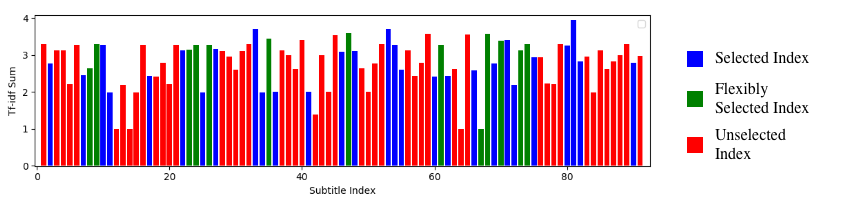
\includegraphics[width=\textwidth]{Legend}
\caption{Plot of selected, flexibly selected indices and unselected indices and their Tf-idf sums for the video from Table~\ref{stellar}}
\label{fig:stellar}
\end{figure*}

\begin{table}[!htpb]
\caption{Results for a 26 minute educational video chosen from NPTEL}
\label{nptel}
\resizebox{\columnwidth}{!}{\begin{tabular}{|c|c|c|c|c|c|c|}
\hline
S. No & Video Title           & Video Length & Flex. Param. & Video Segments & Quality & Bitrate \\ \hline
1     & Hypothesis testing-II & 26 m 24 s    & 10           & 29             & 1080p   & 896k    \\ \hline
\end{tabular}}\vspace{5mm}
\resizebox{\columnwidth}{!}{\begin{tabular}{|l|l|l|l|l|l|}
\hline
Encoder            & Bitrate & Text Learning Time (s) & Video gen. Time (s)          & Time (mins)                       & Final Length of Output           \\ \hline
h264\_videotoolbox & 750k    & 2.63                   & \cellcolor[HTML]{67FD9A}1451 & \cellcolor[HTML]{67FD9A}24 m 11 s & \cellcolor[HTML]{67FD9A}9 m 29 s \\ \hline
\end{tabular}}
\end{table}

\begin{figure*}[!htpb]
\centering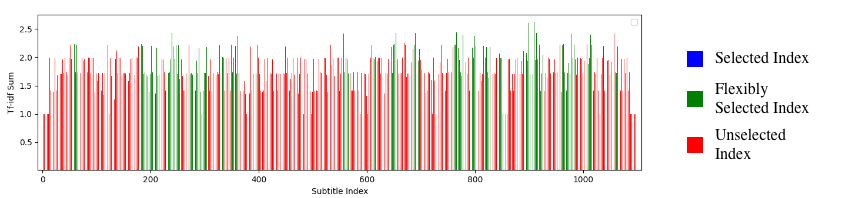
\includegraphics[width=\textwidth]{NPTEL}
\caption{Plot of selected, flexibly selected indices and unselected indices and their Tf-idf sums for the video from Table~\ref{nptel}}
\label{fig:nptel}
\end{figure*}